%%% LaTeX Template: Article/Thesis/etc. with colored headings and special fonts
%%%
%%% Source: http://www.howtotex.com/
%%% Feel free to distribute this template, but please keep to referal to http://www.howtotex.com/ here.
%%% February 2011
%%%
%%% Last updated September 2018 by CDM

%%%  Preamble
\documentclass[11pt,letterpaper]{article}
\usepackage[margin=1.0in]{geometry}
\usepackage[T1]{fontenc}
\usepackage[bitstream-charter]{mathdesign}
\usepackage[latin1]{inputenc}					
\usepackage{amsmath}						
\usepackage{xcolor}
\usepackage{cite}
\usepackage{hyphenat}
\usepackage{graphicx}
\usepackage{float}
\usepackage{subfigure}
\usepackage{sectsty}
\usepackage[compact]{titlesec} 
\usepackage[tablegrid]{vhistory}
\allsectionsfont{\color{accentcolor}\scshape\selectfont}

%%% Definitions
\definecolor{accentcolor}{rgb}{0.0,0.0,0.5} 
\newcommand{\teamname}{3.14159}
\newcommand{\productname}{Traffic Pi}
\newcommand{\coursename}{CSE 4316: Senior Design I}
\newcommand{\semester}{Fall 2018}
\newcommand{\docname}{Project Charter}
\newcommand{\department}{Department of Computer Science \& Engineering}
\newcommand{\university}{The University of Texas at Arlington}
\newcommand{\authors}{Jacob Devasier \\ Ethan Duff \\ Miguel Fraire \\ Kevin Tiller \\ Seth Tisbi}

%%% Headers and footers
\usepackage{fancyhdr}
	\pagestyle{fancy}						% Enabling the custom headers/footers
\usepackage{lastpage}	
	% Header (empty)
	\lhead{}
	\chead{}
	\rhead{}
	% Footer
	\lfoot{\footnotesize \teamname \ - \semester}
	\cfoot{}
	\rfoot{\footnotesize page \thepage\ of \pageref{LastPage}}	% "Page 1 of 2"
	\renewcommand{\headrulewidth}{0.0pt}
	\renewcommand{\footrulewidth}{0.4pt}

%%% Change the abstract environment
\usepackage[runin]{abstract}			% runin option for a run-in title
%\setlength\absleftindent{30pt}			% left margin
%\setlength\absrightindent{30pt}		% right margin
\abslabeldelim{\quad}	
\setlength{\abstitleskip}{-10pt}
\renewcommand{\abstractname}{}
\renewcommand{\abstracttextfont}{\color{accentcolor} \small \slshape}	% slanted text

%%% Start of the document
\begin{document}

%%% Cover sheet
{\centering \huge \color{accentcolor} \sc \textbf{\department \\ \university} \par}
\vspace{1 in}
{\centering \huge \color{accentcolor} \sc \textbf{\docname \\ \coursename \\ \semester} \par}
\vspace{0.5 in}
\begin{figure}[h!]
	\centering
   	
\includegraphics[width=0.45\textwidth]{images/traffic_light}
\end{figure}
\vspace{0.5 in}
{\centering \huge \color{accentcolor} \sc \textbf{\teamname \\ \productname} \par}
\vspace{0.5 in}
{\centering \large \sc \textbf{\authors} \par}
\newpage


%\vspace{1 in}
%\centerline{January 13th, 2012}
%\newpage

%%% Revision History
\begin{versionhistory}
  	\vhEntry{0.1}{09.28.2018}{JD|ED|MF|KT|ST}{document creation}
  	\vhEntry{0.2}{10.03.2018}{JD|ED|MF|KT|ST}{complete draft}
  	\vhEntry{1.0}{12.03.2018}{JD|ED|MF|KT|ST}{error correction}
  	%%%\vhEntry{0.3}{10.12.2018}{AT|GH}{release candidate 1}
  	%%%\vhEntry{1.0}{10.20.2018}{AT|GH|CB}{official release}
  	%%%\vhEntry{1.1}{10.31.2018}{AL}{added customer change requests}
\end{versionhistory}
\newpage

%%% Table of contents
\tableofcontents
\newpage

%%% List of figures and tables (optional)
\listoffigures
%\listoftables
\newpage
\setcounter{table}{0}

%%% Agile project charter sections
\section{Vision}
The current system process for conducting initiating, conducting, and utilizing traffic studies involves an appeal from the citizens of a particular neighborhood to the city, an expensive ‘pneumatic road tube’ for measuring traffic, and the subsequent placement of speed bumps, stop signs, or signal lights for what may be just a rogue driver. This project aims to empower the citizen to conduct their own traffic study at fraction of the cost of the traditional method, provide the city with an efficient and cost effective alternative to the traditional method, provide more information on the vehicles in the traffic study, and utilize a crowd sourced repository of traffic data to improve traffic conditions in a neighborhood or city as a whole.
\section{Mission}
To circumvent the traditional approach to a traffic study, the team envisions a solution that uses a micro-controller controller camera unit that can be mounted on tripod or attached to the side of a house. The camera will record in real time the traffic flow at an intersection, thoroughfare, or area of interest to the traffic study. Using an object recognition program along with analysis of pixel data, the speed of vehicles passing through the cameras vision will be monitored. This data will be sent to a centralized cloud server that will be able to run increased analytics on the vehicle, taking the raw data of speed, direction, etc. and outputting a user friendly report based the input data.
\section{Success Criteria}
The success of this project will be determined by a number of milestones listed below.
\\
\\
At the end of nine month design and development period success will of the project will be assessed based on if the following criteria have been met:
\begin{itemize}
  \item The system is able to accurately determine the speed of a vehicle within its field of view
  \item The system is able to reliably perform for at least one week
  \item The overall cost of the system is within \$800 dollars
  \item The system is able to output the data in a user friendly format
\end{itemize}
\\
Within 12 months after the prototype has been designed and developed these success indicators will be used:
\begin{itemize}
  \item The system will be able filter anything except vehicles out of its input data
  \item The system will be able to transfer the data on its computer to a cloud server
  \item The system will be able to perform increased analytics on the data in the cloud server
  \item The system will be able to interface with a mobile device
  \item The system will be able to generate a traffic model of the area of interest
\end{itemize}
\\
Within 16 months after the prototype delivery date, we expect the following success indicators to be observed:
\begin{itemize}
  \item The overall cost of the system being reduced by \%15
  \item The system will be able to connect to other deployed systems, thereby monitoring a wider area
  \item The system will be able to generate a traffic model of multiple areas of interest and their possible correlations
\end{itemize}
\newpage

%%% Remaining project charter sections
\section{Background}
The current method by which a traffic study takes place can be generalized by the following. A need for such a study arises in a neighborhood (multiple accidents over a period of time at a particular intersection, multiple close-calls at a particular intersection, etc.). Either the city recognizes a potential problem in the area of interest or a resident in the community makes known to the city the area and requests something be done. The city will usually follow up on the request with a traffic study; monitoring the area with pneumatic road tubes, wires laid on the ground that monitor the speed a of vehicle as it passes over it. Depending on the area of interest, multiple road tubes may be used along with other equipment or actual persons on the ground monitoring the area. After the area has been monitored for a given period of time a decision is made on the area (install stop sign, signal lights, road bump, etc.). There are several problems with the current model.

To begin, the ultimate decision to initiate a traffic study begins with the city. A citizen, neighborhood, or even business park may request/petition the city to investigate potentially dangerous area but these are only requests. If in fiscally troubling times the funds for such a study are lacking, the study may not even be feasible and thus not occur. Additionally if the city for whatever reason (politically motivated, not enough complaints, etc.) decides not to investigate the area, the public is not able to have their request satisfied. 

If a city does decide to begin a traffic study, the cost of such a study may limit the scope or duration of the study. On average the cost of a single pneumatic road tube can range from \$500 to the \$1000's. This cost does not include the installation cost, environment hazards, maintenance, and otherwise. This cost is heavy on both large and small cities. In large cities, there is likely an abundance of areas that require a traffic study and thus multiple devices must be deployed. In small cities the budget for such a device may not exist at all. In short, the cost of the current method is high.

Lastly, in relating to the above two points, the ability to perform the study lies solely within the city because of power and money. The individual citizen, neighborhood, or entity is not able due to the reasons above able to conduct this study on their own. Relegating what should be a local affair to city governance. 
\section{Related Work}
The current state of the traffic study arena is mainly focused on using existing traffic cameras and performing traffic analysis on it. For example, Logipix Technical Development Ltd. is a company that specializes in high-end video surveillance solutions (Logipix, 2017). This company uses professional grade cameras to monitor airports, highways, stadiums, or big areas of interest. Another company TrafficVision specializes in analyzing prerecorded footage for customers and provided specific data reports for them (TrafficVision, 2018). 

Aside from the above two, there are currently two companies that have similar products to what this team is trying to achieve. 

The first is Miovision Technologies Inc. This company speciliazes in a broad area for performing traffic studies. They are able to capture video of intersections, park trails, neighborhoods, crosswalks, and more. The data is analyzed and presented to the customer in a concise usable format for making traffic decisions (Miovision, 2018). The company can use the existing cameras placed by the city or deploy its own equipment on site. 

The second company is Roadometry. This company is similar to Miovision in that it can deploy its own camera systems, record, traffic, and analyze it as well (Roadometry, 2018).

The difference between the products and solutions these companies offer and the direction this team is taking with the Traffic Pi project is that, their solutions are marketed to city customers with correpsonding price tags. The Traffic Pi aims to market to individual homeowners or neighborhoods.
\section{System Overview}
The architecture revolves primarily around the raspberry pi computer itself.  The interface of the raspberry pi will communicate with all other major systems sending commands and receiving data.  The first major system to communicate with is the vision system.  This system is responsible for the cameras and has two that are part of it: the IR camera, and the 3D camera.  Both will connect to the PI's interface in order to transmit visual data.  This data will be redirected by the interface to the Pre-processing unit which will determine what raw film data is worth keeping and what is not by a factor of cars in the streets.  Data kept is placed into storage which the interface can then pull out again.  It is powered by a socket connected to the power system, an outlet inside the users home.  The case system has a cooling unit which prevents the PI from overheating through a ventilation shaft.  This fan draws power from the PI via its interface.  When the PI is connected to the user's computer via Ethernet, it will automatically run its application on their computer.  This application receives transferred data from the PI's storage and processes it, splitting meta data into a database and film data into local storage.  All of this data will be accessible to the user via a graphic user interface.

\begin{figure}[h!]
	\centering
 	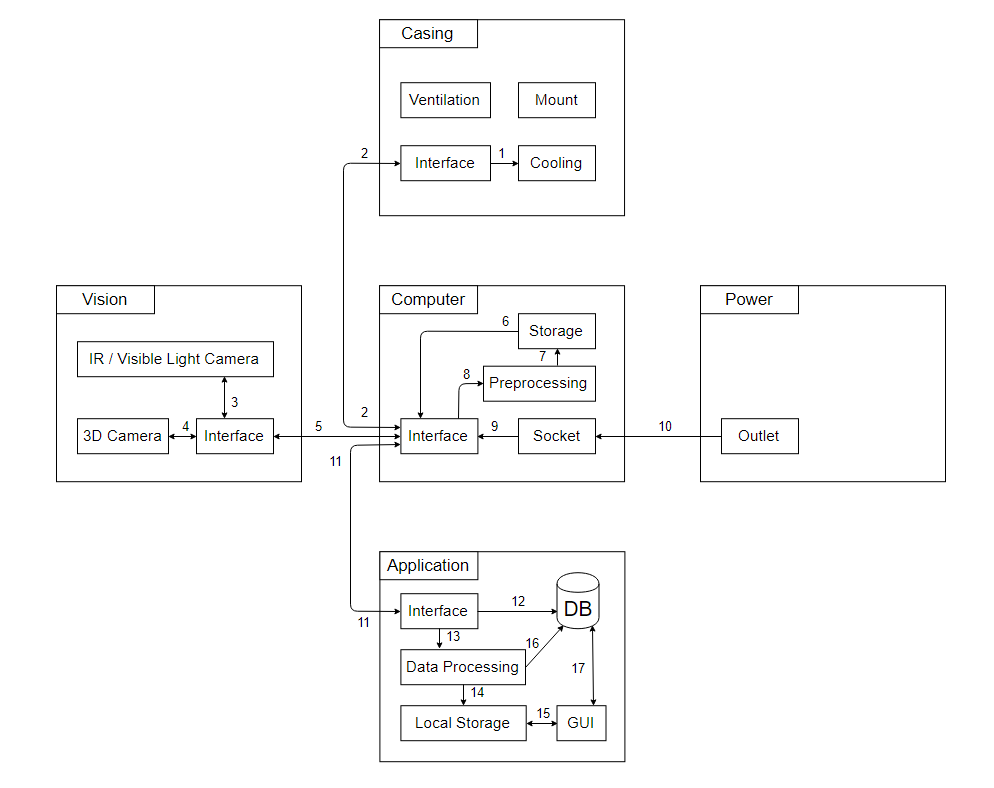
\includegraphics[width=0.60\textwidth]{images/ADS.png}
 \caption{A simple architectural layer diagram}
\end{figure}

\subsection{Layer Computer Description}
The main purpose of the computer layer is to the central source of communication and serve as the collector and organizer of data received from the vision layer. Maintaining power granted by the power layer and distribute to the cooling system, cameras, and itself to function as desired. Allowing to request proper cooling from the case layer to maintain functionality of the Traffic Pi without worrying about unstable temperature both generated from internal and environmental. The computer layer will take in raw data from the vision layer, such as footage (frames), distance, and lighting, after detecting cars passing by. Pre-processing will take in effect, time stamping frames and formatting data, then direct to the storage for later use by the application layer.

\subsection{Layer Vision Description}
The vision layer comprises of the physical cameras, IR / visible light and 3D cameras, that views the road and transmit the footage data to the Traffic Pi's pre-processing and stored for later. The IR / visible light camera would be able to view the road and passing vehicles in both day and night settings. The 3D camera will be able to measure the distance of the passing vehicles from the camera in every passing frames. While collecting data, until function completion is met, the footage / frames and distance will to send to the computer layer.

\subsection{Layer Application Description}
The main purpose of the application layer is to handle the actual processing of the raw video on the users local machine coming from the computer layer. During the video processing, bounding boxes will be placed around every appropriate vehicle and speed will be measured and recorded. The resulting data will be stored on a local database. Meanwhile, the resulting video will be stored on the users local storage. This layer provides the user with a graphical user interface in order to interact with the system. Using the GUI, the user will be able to view the analyzed video and will have the option be presented with a dashboard fitted with the visual representation of the analytics regarding the traffic study. The user will also have the option of a quick guide and options to download the file of data.

\subsection{Layer Case Description}
The case layer is designed to house every component in a self contained physical structure. The case is designed such that the heat generated from the Raspberry Pi, IR camera, and 3D camera will be able to dissipate quickly away from the system. This ventilation works in conjunction with the cooling subsystem. The cooling component is a small fan that will be attached to the case layer and provide additional temperature control to the Traffic Pi system as a whole. Both the ventilation and cooling component of the case layer are designed to minimize the effects of heat generation on the system. Although the ventilation subsystem is simply a built-in designed component of the case, it is referred to as its own subsystem as it has its own unique functionality. The case layer also includes a mounting plate subsystem which is a physical component designed to make mounting of the Traffic Pi system on a tripod or other auxiliary surface easier. Finally, a USB Type C cable called the interface is the last subsystem designated as part of the case layer. This component is responsible for running power from the Raspberry Pi to the cooling fan subsystem.

\subsection{Layer Power Description}
The power layer is specified for explicit visualization of the providing power to the system. This layer consists of only one subsystem, the outlet. Outlet is defined as any US AC power outlet providing 120V at 60Hz. A power cable is run from this outlet to the Raspberry Pi to provide power to it and by extension each of the other layers. 
\section{Roles \& Responsibilities}
As this project is the brain child of Dr. McMurrough, he is the only actual stakeholder in this endeavour. The product that is being developed is still only a prototype and has no committed customer that can be relied considered a stakeholder. As such, the team, over the course development cycle, will interact directly with Dr. McMurrough on developing a firm direction and tangible requirements that the system will have. 

The team consists of Ethan Duff, Jacob Devasier, Kevin Tiller, Miguel Fraire, and Seth Tisbi. There are no specific roles that have been assigned to any team member. Each member is resonsible in equal part for all development that will take place.

The roles of product owner and scrum master will be rotated through the team, allowing each member to own the responsibility that comes with the role.
\section{Cost Proposal}
The biggest expense the team will encounter is the video graphics card in order to handle some heavy processing. Everything else is relatively affordable. The team does not expect to come anywhere close to exceeding the budget.

\subsection{Preliminary Budget}

\begin{table}[h]
\centering
\resizebox{.65\textwidth}{!}{%
\begin{tabular}{|l|l|1|1|}
\hline
 \textbf{Description} & \textbf{Credits} & \textbf{Debits} & \textbf{Balance}\\ \hline
Allotted budget & 800.00 && \\ \hline
Raspberry Pi && 37.00& \\ \hline
Micro SD card && 15.00&\\ \hline
Geforce GTX 1050 && 150.00 &\\ \hline
Arducam Noir Camera && 30.00&\\ \hline
3D printing filament && 15.00&\\ \hline
Cloud service && 14.60/month&\\ \hline
External Hard drive && 35.00& \\ \hline
Tri-pod && 42.00& \\ \hline
\textbf{Total} & 800.00 & -338.60 & 461.40  \\ \hline
\end{tabular}}
\caption{High level budget table} 
\end{table}

\subsection{Current \& Pending Support}
As of now and into the foreseeable future Traffic Pi will only have one funding source. It is comprised solely of the default eight hundred dollar amount granted by the CSE department.
\section{Facilities \& Equipment}
The team anticipates spending some time in the senior deign lab using the 3D printing equipment. We have intentions of designing and prototyping a secure and weatherproof enclosure for our components (Raspberry Pi, camera, backup battery, ect...). Regarding testing grounds for our equipment, it is possible that the Traffic Pi could be initially tested at a parking lot. Eventually, the Traffic Pi will have to tested in some residential neighborhood. Once initial testing is complete the plan consists of visiting one of these neighborhoods to ask a few residents for their permission to deploy the Traffic Pi equipment outside of their house for a given amount of time. If this doesn't work out, we could always ask the university to for their permission to deploy the Traffic Pi somewhere on campus.
\section{Assumptions}
\begin{itemize}
  \item A suitable outdoor testing location will be available by the 3rd sprint cycle
  \item All of the components will be fully functional
  \item Access to the installation site will be granted by the 4th sprint cycle
  \item There will be a reliable power source and network connectivity at the deployment site
  \item The network infrastructure at the deployment site will allow TCP network traffic on port 8080
\end{itemize}
\section{Constraints}
\begin{itemize}
  \item Final prototype demonstration must be completed by May 1st, 2019
  \item A volunteering citizen must be willing to allow on-site outdoor deployment and use of their power source along with network connectivity 
  \item The deployment site will only be accessible by the development team during normal business hours
  \item Total development costs must not exceed \$800
  \item All data obtained from the Traffic Pi must remain confidential and must never be made public.
\end{itemize}

\section{Risks}
\begin{table}[h]
\resizebox{\textwidth}{!}{
\begin{tabular}{|l|l|l|l|}
\hline
 \textbf{Risk description} & \textbf{Probability} & \textbf{Loss (days)} & \textbf{Exposure (days)} \\ \hline
 Memory loss/corruption  & 0.20 & 6 & 2.0 \\ \hline
 Outdoor testing grounds are not available  & 0.30 & 18 & 3.5 \\ \hline
 Internet access not available at deployment site  & 0.30 & 9 & 2.7 \\ \hline
 Weather damage  & 0.10 & 15 & 2.0 \\ \hline
 Theft & 0.15 & 12 & 2.5 \\ \hline
\end{tabular}}
\caption{Overview of highest exposure project risks} 
\end{table}
\section{Documentation \& Reporting}
%%% In this section, you will describe all of the various artifacts that you will generate and maintain during the project life cycle. Describe the purpose of each item below, how the content will be generated, where it will be stored, how often it will be updated, etc. Replace the default text for each section with your own description. Reword this paragraph as appropriate.

\subsection{Major Documentation Deliverables}

\subsubsection{Project Charter}

This document will be updated a total of three times. Once towards the beginning of senior design 1, the initial delivery date is October 3rd 2018. The second time will be at the end of senior design 1 and the final version will be delivered towards the end of senior design 2.

\subsubsection{System Requirements Specification}
System Requirements Specification is maintained and updated as the team goes through options and weighs cost and risk. Initial version to be done by sprint 2. Final version to be done by sprint 8.

\subsubsection{Architectural Design Specification}
Architectural Design Specification is maintained and updated as the team makes changes to the design. Initial version to be done by sprint 3. Final version to be done by sprint 8.

\subsubsection{Detailed Design Specification}
Detailed Design Specification is maintained and updated as the team makes changes to the design. Initial version to be done by sprint 5. Final version to be done by sprint 8.

\subsection{Recurring Sprint Items}


\subsubsection{Product Backlog}
Backlog items are voted among the team and added through a majority vote. Items will be prioritized based on how it can meet the requirements for the product, such as a camera. Sprint backlogs will be documented on trello.

\subsubsection{Sprint Planning}
Sprint duration of 2 weeks each. Total of 8 sprints.

\subsubsection{Sprint Goal}
Sprint goals are decided by the team and is determined by what has not been completed the previous sprint and what needs to be complete.

\subsubsection{Sprint Backlog}
Backlog items are voted among the team and added through a majority vote. Sprint backlogs will be documented on trello.

\subsubsection{Task Breakdown}
Team members will claim tasks for themselves with the knowledge and agreement of the rest of the team.  The product owner will not have final say over task delegation.  Time will documented in individual sprints.

\subsubsection{Sprint Burndown Charts}
The team will be mutually responsible for the charts.  The format shall be an x,y line graph.  Slack plugin will be used.

\begin{figure}[h!]
    \centering
    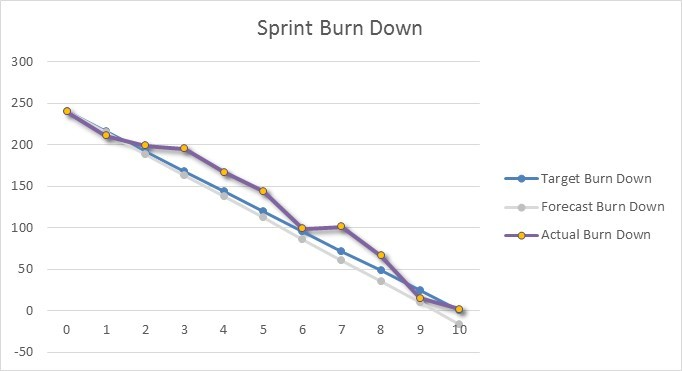
\includegraphics[width=0.7\textwidth]{images/burndownchart}
    \caption{Example sprint burn down chart}
\end{figure}

\subsubsection{Sprint Retrospective}
A meeting after each due sprint will be held immediately after class.  The documentation will be done in the respective engineering notebooks and presentation slides.

\subsubsection{Individual Status Reports}
Whenever a work session is finished, a report will be issued specifying the current progress of assigned tasks.

\subsubsection{Engineering Notebooks}
How often will the engineering notebook be updated, at a minimum, by each team member? What is the minimum amount of pages that will be completed for each interval, and how long will that interval be? How will the team keep each member accountable? Who will sign of as a "witness" for each ENB page?

\subsection{Closeout Materials}

\subsubsection{System Prototype}
The system itself, plus a raspberry pi and camera system, plus a mounting device.  Details of mounting device to be determined.

\subsubsection{Project Poster}
The poster is currently not a prioritized task.  Should it be so in the future, dimensions will be decided upon by the team member assigned this task.

\subsubsection{Web Page}
We will have a web page to provide instructions on how to set up the device and include a demonstration video of how the device works including any important information the user may need to know while using or setting it up. If our group decides to market our product to sell to people, then we will also allow prospective users to purchase the device at a price determined by our team. The web page will be under construction throughout the developmental sprints, but we would like to have some introductory information regarding what we are doing and how we plan to do it posted before then.

\subsubsection{Demo Video}
In our product demonstration video, we will show off what our product is, how it works, and what we hope to accomplish with it. Included in our demonstration video will be information including, but not limited to, how to set it up, how to use it, what information it will be collecting, and any problems we would like to solve with our product.

\subsubsection{Source Code}
Our team’s code will be managed on a team GitHub account that we each have access to. Each member will clone the directory to their personal machine and will commit changes through each members personal GitHub account. Because our product has market potential, we would like to use a private GitHub repository to prevent members outside of our team from accessing our code.
If we do market our product, the customer should be provided access to execute the code and manage any configuration we allow; otherwise, we will keep our product private.

\subsubsection{Source Code Documentation}
While we are still considering other options, we will most likely use Doxygen to manage our source code documentation. Once we have begun work on the development, we will solidify our choice. This way, we will know exactly which languages we will need support for and we will be able to determine our best choice for documentation. We would like to be able to export the source code to a web format that is browsable by the team. Because of this preference, we have chosen Doxygen as it supports exporting to HTML.

\subsubsection{Hardware Schematics}
Because our product is mostly software-based, we will not have much hardware integration to include. Currently, our plan is to use a camera with an infrared and visible light sensor to track any passing vehicles and mount it along with a Raspberry Pi and any other hardware components inside a case. 

\subsubsection{CAD files}
Our product will likely be housed inside of a 3D printed container. To design the housing for everything, we will use one of the many free 3D modelling software available. STL seems to be the best format to save our 3D designs as, so we will be using it to send to the 3D printer.

\subsubsection{Installation Scripts}
Along with our product, we will provide installation instructions to provide the user with simple installation instructions. Should we decide to implement an auto-installer, we will provide the necessary installation information during the installation phase. We will know more about this part when we begin the software implementation of our product.

\subsubsection{User Manual}
The user will be provided information on how to run and use the product in multiple forms. We will allow the user to access our user manual through our web page, which will also contain an installation and demonstration video. 
Along with this, we will provide an offline version of our user manual included with the software or packaged with the product itself. Should the user need any help setting it up, we hope to provide a help page included in the user manual and on the website.
\newpage

%%% References
\bibliographystyle{plain}
\bibliographystyle{reference/IEEEtran_custom}
\bibliography{reference/refs}{}

\end{document}